%
% teil2.tex -- Beispiel-File für teil2 
%
% (c) 2020 Prof Dr Andreas Müller, Hochschule Rapperswil
%
% !TEX root = ../../buch.tex
% !TEX encoding = UTF-8
%
\section{Riemannsche Zeta-Funktion}\label{Riemannsche Zeta-Funktion}

Die Riemannsche Zeta-Funktion wurde 1859 von Bernhard Riemann untersucht und ist eine zentrale Funktion der
analytischen Zahlentheorie. Sie wird üblicherweise als unendliche Reihe
definiert. Für alle komplexen Variablen s mit Realteil grösser als 1
ergibt sich ihre Darstellung als
\[
\zeta(s) = \sum_{n = 1}^{\infty}\frac{1}{n^{s}}.
\]
Diese Definition beschreibt eine Dirichlet-Reihe, deren Konvergenz für Re(s) \textgreater{} 1 gewährleistet ist. 
Bereits in diesem Definitionsbereich zeigt die Funktion bemerkenswerte Eigenschaften. 
So nimmt sie für bestimmte Argumente konkrete Werte an:

\begin{table}[h]
	\centering
	\begin{tabular}{|c|c|c|}
		\hline
		\rowcolor{blue!40}
		\textcolor{white}{\textbf{\textit{s}}} & 
		\textcolor{white}{\textbf{$\zeta(s)$}} & 
		\textcolor{white}{\textbf{Ungefährer Wert}} \\
		\hline
		$2$ & $\pi^2/6$ & $\approx 1{,}6449$ \\
		\hline
		$4$ & $\pi^4/90$ & $\approx 1{,}0823$ \\
		\hline
		$-1$ & $-1/12$ & (analytische Fortsetzung) \\
		\hline
		$0$ & $-1/2$ & (analytische Fortsetzung) \\
		\hline
	\end{tabular}
	\caption{Ausgewählte Werte der Zeta-Funktion}
	\label{tab:zeta}
\end{table}

Besonders bemerkenswert ist hier der Wert $\zeta$(2) = $\frac{\pi^2}{6}$, den Euler bereits 1735 nachwies, bekannt als das Basler Problem. 
Die letzen beiden Zeilen der Tabelle gehören jedoch nicht zum ursprünglichen Definitionsbereich (s > 1), sondern sind nur durch analytische Fortsetzung erreichbar. 

\begin{figure}
	\centering
	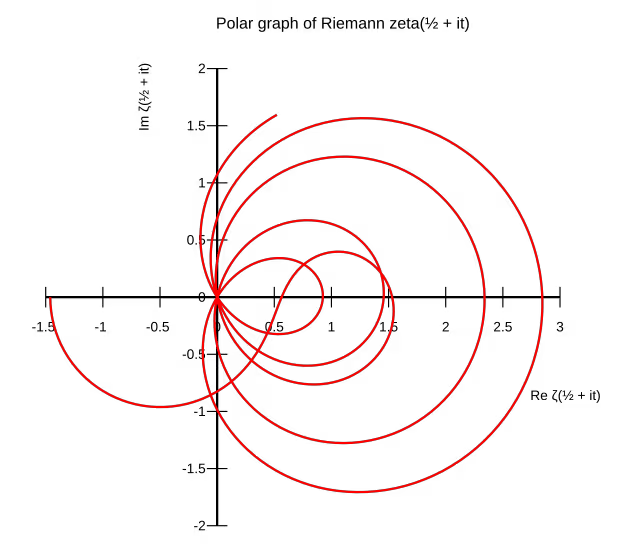
\includegraphics[width=0.7\linewidth]{papers/zeta/Abbildung_Zeta.png}
	\caption{}
	\label{fig:abbildungzeta}
\end{figure}

Die spiralförmige Darstellung in Abbildung \ref{fig:abbildungzeta} zeigt den Verlauf der Zeta-Funktion $\zeta$(s) in der komplexen Ebene, wobei s entlang einer vertikalen Linie mit festem Realteil variiert. Die Schnittpunkte der Kurve mit dem Ursprung (sichtbar als die Stellen, an denen die Spirale durch den Mittelpunkt verläuft) entsprechen den sogenannten nicht-trivialen Nullstellen der Zeta-Funktion. Diese liegen alle auf der Linie Re(s) = $\frac{1}{2}$ und sind Gegenstand der berühmten, bis heute unbewiesenen Riemannschen Vermutung, einem der bedeutendsten offenen Probleme der Mathematik. 

Nützlich ist die Riemannsche Zeta-Funktion ebenfalls, um eine Annäherung der Primzahlfunktion zu schaffen. 
Das Euler-Produkt
\[
\zeta(s) = \prod_{p \ \text{prim}} \frac{1}{1 - p^{-s}}
\]
beschreibt eine geometrische Reihe,welche den Zusammenhang aller Primzahlen aufzeigt. 

\begin{figure}
	\centering
	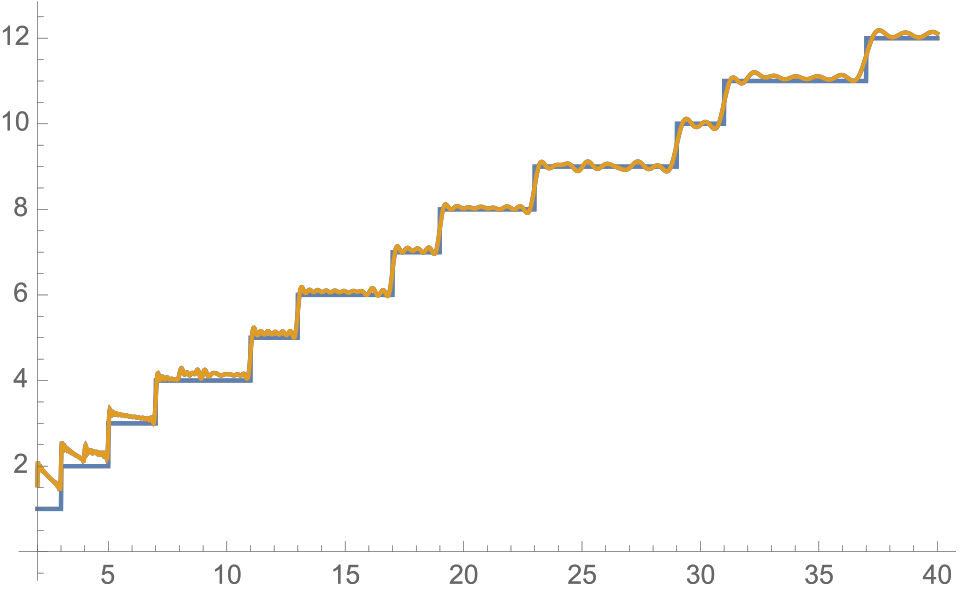
\includegraphics[width=0.7\linewidth]{papers/zeta/Primzahlen.png}
	\caption{}
	\label{fig:primzahlen}
\end{figure}

Die blaue Treppenkurve in Abbildung \ref{fig:primzahlen} zeigt die Primzahlzählfunktion $\pi$(x), welche für jede reelle Zahl x angibt, wie viele Primzahlen kleiner oder gleich x existieren. Die orangefarbene Kurve stellt den Logarithmischen Integralausdruch Li(x) dar. Das ist eine von Riemann entwickelte Näherungsformel für $\pi$(x), die direkt aus der Zeta-Funktion abgeleitet wird. Man erkennt deutlich, wie eng beide Kurven beieinander liegen: Li(x) approximiert die Verteilung der Primzahlen mit bemerkenswertet Genauigkeit, selbst für kleine Werte von x.



% Für was wird die Zeta-funktion angewendet in der Praxis? -> Verteilung von Primzahlen, analytische Zahlentheorie, mathematische Physik und Wahrscheinlichkeit und Statistik
% Text zum Bild schreiben
% Abstimmen auf Text vom Theorieteil des Buches von Herr Müller. Erweiterung mit Primzahl-Funktion. 

